\documentclass{standalone}
\usepackage[utf8]{inputenc}
\usepackage{tikz}
\usetikzlibrary{shapes.geometric, arrows}
\usetikzlibrary{calc}

\tikzset{block/.style = {rectangle, thick, minimum width=3cm, minimum height=1cm, text centered, text width=3cm, draw=black}}
\tikzset{io/.style = 	{trapezium, trapezium left angle=70, trapezium right angle=-70, trapezium stretches=true, thick, minimum width=3cm, minimum height=1cm, text centered, text width=3cm, draw=black}}
\tikzset{arrow/.style = {thick,->,>=stealth}}

\begin{document}
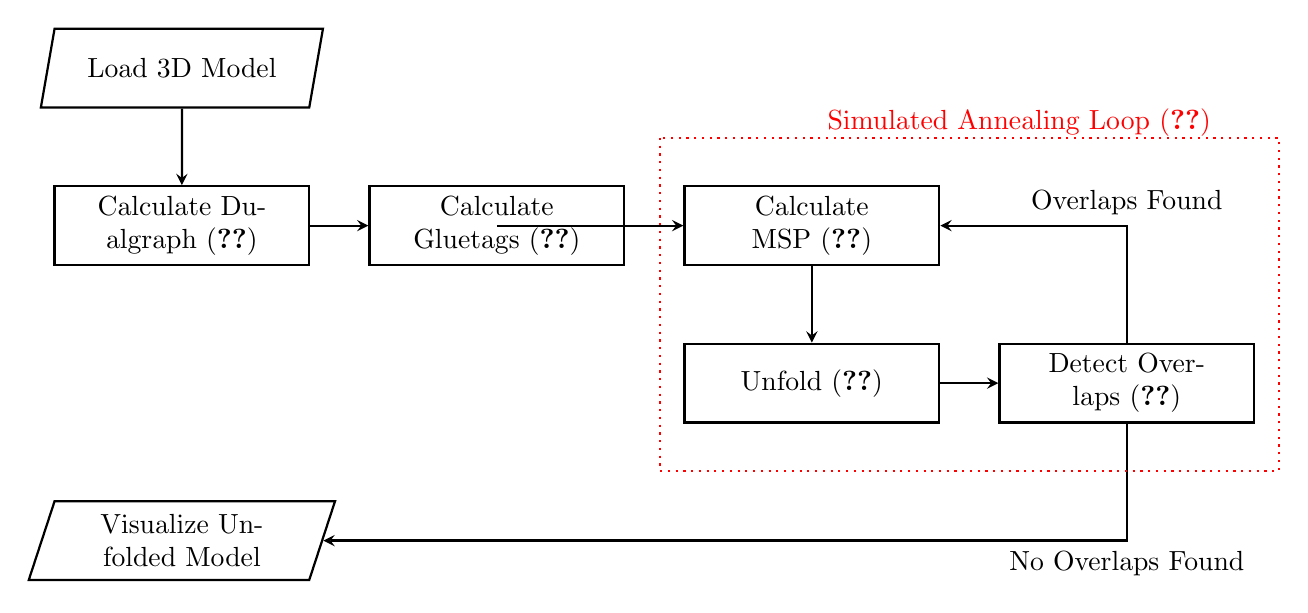
\begin{tikzpicture}[node distance=2cm]
	\node (load) 	[io]									{Load 3D Model};
	\node (cd) 		[block, below of=load] 					{Calculate Dualgraph (\ref{sec:calcdual})};
	\node (cgt)	 	[block, right of=cd, xshift=2cm] 		{Calculate Gluetags (\ref{sec:calcgluetag})};
	\node (msp) 	[block, right of=cgt, xshift=2cm] 		{Calculate MSP (\ref{sec:calcmsp})};
	\node (unfold) 	[block, below of=msp] 					{Unfold  (\ref{sec:unfold})};
	\node (od)		[block, right of=unfold, xshift=2cm] 	{Detect Overlaps  (\ref{sec:overlaps})};
	\node (finish) 	[io, below of=cd, yshift=-2cm]			{Visualize Unfolded Model};
	
	\draw [arrow] (load) 	-- (cd);	
	
	\draw [arrow] (cd) 		-- (cgt);
	\draw [arrow] (cgt) 	|- (msp);
	\draw [arrow] (msp) 	-- (unfold);
	\draw [arrow] (unfold) 	-- (od);
	
	\draw [arrow] (od) 		|- node[anchor=north] {No Overlaps Found} 	(finish);
	\draw [arrow] (od) 		|- node[anchor=south] {Overlaps Found} 		(msp);
	
	\draw[red,thick,dotted] ($(msp.north west)+(-0.3,0.6)$) node[right, yshift=0.2cm, xshift=2cm] {Simulated Annealing Loop (\ref{sec:annealing})} rectangle ($(od.south east)+(0.3,-0.6)$);
\end{tikzpicture}
\end{document}